%% (Master) Thesis template
% Template version used: v1.4
%
% Largely adapted from Adrian Nievergelt's template for the ADPS
% (lecture notes) project.



%% We use the memoir class because it offers a many easy to use features.
\documentclass[11pt,a4paper,table,hidelinks]{memoir}  % Remove "hidelinks" for red boxes around hyperlinks

%% Packages
%% ========

%% LaTeX Font encoding -- DO NOT CHANGE
\usepackage[OT1]{fontenc}

%% Babel provides support for languages.  'english' uses British
%% English hyphenation and text snippets like "Figure" and
%% "Theorem". Use the option 'ngerman' if your document is in German.
%% Use 'american' for American English.  Note that if you change this,
%% the next LaTeX run may show spurious errors.  Simply run it again.
%% If they persist, remove the .aux file and try again.
\usepackage[english]{babel}

%% Input encoding 'utf8'. In some cases you might need 'utf8x' for
%% extra symbols. Not all editors, especially on Windows, are UTF-8
%% capable, so you may want to use 'latin1' instead.
\usepackage[utf8]{inputenc}

%% This changes default fonts for both text and math mode to use Herman Zapfs
%% excellent Palatino font.  Do not change this.
%\usepackage[sc]{mathpazo}

%% The AMS-LaTeX extensions for mathematical typesetting.  Do not
%% remove.
\usepackage{amsmath,amssymb,amsfonts,mathrsfs}

%% NTheorem is a reimplementation of the AMS Theorem package. This
%% will allow us to typeset theorems like examples, proofs and
%% similar.  Do not remove.
%% NOTE: Must be loaded AFTER amsmath, or the \qed placement will
%% break
\usepackage[amsmath,thmmarks]{ntheorem}

%% LaTeX' own graphics handling
\usepackage{graphicx}

%% We unfortunately need this for the Rules chapter.  Remove it
%% afterwards; or at least NEVER use its underlining features.
\usepackage{soul}

%% This allows you to add .pdf files. It is used to add the
%% declaration of originality.
\usepackage{pdfpages}

\newenvironment{conditions}
  {\par\vspace{\abovedisplayskip}\noindent\begin{tabular}{>{$}l<{$} @{${}={}$} l}}
  {\end{tabular}\par\vspace{\belowdisplayskip}}

%% Some more packages that you may want to use.  Have a look at the
%% file, and consult the package docs for each.
%% See the TeXed file for more explanations

%% [OPT] Multi-rowed cells in tabulars
%\usepackage{multirow}

%% [REC] Intelligent cross reference package. This allows for nice
%% combined references that include the reference and a hint to where
%% to look for it.
\usepackage{varioref}

%% [OPT] Easily changeable quotes with \enquote{Text}
%\usepackage[german=swiss]{csquotes}

%% [REC] Format dates and time depending on locale
\let\ordinal\relax %% prevent warning
\usepackage{datetime}

%% [OPT] Provides a \cancel{} command to stroke through mathematics.
%\usepackage{cancel}

%% [NEED] This allows for additional typesetting tools in mathmode.
%% See its excellent documentation.
\usepackage{mathtools}

%% [NEED] Conditional commands
\usepackage{ifthen}

%% [OPT] Manual large braces or other delimiters.
%\usepackage{bigdelim, bigstrut}

%% [REC] Alternate vector arrows. Use the command \vv{} to get scaled
%% vector arrows.
\usepackage[h]{esvect}

%% [NEED] Some extensions to tabulars and array environments.
\usepackage{array}

%% [OPT] Postscript support via pstricks graphics package. Very
%% diverse applications.
%\usepackage{pstricks,pst-all}

%% [?] This seems to allow us to define some additional counters.
%\usepackage{etex}

%% [ADV] XY-Pic to typeset some matrix-style graphics
%\usepackage[all]{xy}

%% [OPT] This is needed to generate an index at the end of the
%% document.
%\usepackage{makeidx}

%% [OPT] Fancy package for source code listings.  The template text
%% needs it for some LaTeX snippets; remove/adapt the \lstset when you
%% remove the template content.
\usepackage{listings}
% \lstset{language=TeX,basicstyle={\normalfont\ttfamily}}

%% [REC] Fancy character protrusion.  Must be loaded after all fonts.
%\usepackage[activate]{pdfcprot}

%% [REC] Nicer tables.  Read the excellent documentation.
\usepackage{booktabs}

%% [OPT] Package for adding TODOs.
\usepackage{todonotes}

%% [OPT] Package to define and use acronyms
\usepackage[nolist,nohyperlinks,smaller]{acronym}
 

%% Our layout configuration.  DO NOT CHANGE.
%% Memoir layout setup

%% NOTE: You are strongly advised not to change any of them unless you
%% know what you are doing.  These settings strongly interact in the
%% final look of the document.

% Dependencies
%\usepackage{ETHlogo}

% use helvetica as default font:
\usepackage[scaled]{helvet}
%\renewcommand\familydefault{\sfdefault} 

% Turn extra space before chapter headings off.
\setlength{\beforechapskip}{0pt}

\nonzeroparskip
\parindent=0pt
\defaultlists

% Chapter style redefinition
\makeatletter

\makepagestyle{headerWPageNr}% Create headerWPageNr style
\if@twoside
  \copypagestyle{headerWPageNr}{Ruled}
  \copypagestyle{chapter}{Ruled}
\else
  \copypagestyle{headerWPageNr}{ruled}
  \copypagestyle{chapter}{ruled}
\fi
% chapter pages have no header and center page number in footer:
\makeoddhead{chapter}{}{}{}
\makeevenhead{chapter}{}{}{}
\makeoddfoot{chapter}{}{\thepage}{}
\makeevenfoot{chapter}{}{\thepage}{}
\makeheadrule{chapter}{\textwidth}{0pt}

% all other pages have page number and chapter or section name in header without footer:
\makeoddhead{headerWPageNr}{\rightmark}{}{\thepage}
\makeevenhead{headerWPageNr}{\thepage}{}{\leftmark}
\makeoddfoot{headerWPageNr}{}{}{}
\makeevenfoot{headerWPageNr}{}{}{}
\pagestyle{headerWPageNr}% Set page style to headerWPageNr


\makechapterstyle{bianchimod}{%
  \copypagestyle{abstract}{empty}
  \chapterstyle{default}
  \renewcommand*{\chapnamefont}{\normalfont\Large\sffamily}
  \renewcommand*{\chapnumfont}{\normalfont\Large\sffamily}
  \renewcommand*{\printchaptername}{%
    \chapnamefont\centering\@chapapp}
  \renewcommand*{\printchapternum}{\chapnumfont {\thechapter}}
  \renewcommand*{\chaptitlefont}{\normalfont\huge\sffamily}
  \renewcommand*{\printchaptertitle}[1]{%
    \hrule\vskip\onelineskip \centering \chaptitlefont\textbf{\vphantom{gyM}##1}\par}
  \renewcommand*{\afterchaptertitle}{\vskip\onelineskip \hrule\vskip
    \afterchapskip}
  \renewcommand*{\printchapternonum}{%
    \vphantom{\chapnumfont {9}}\afterchapternum}}
  
\makechapterstyle{bianchimod2}{%
  \renewenvironment{abstract}{\chapter*{\abstractname}}{}
  \chapterstyle{default}
  \definecolor{ChapGrey}{rgb}{0.6,0.6,0.6}
  \newcommand{\LargeFont}{% Needs a ’stretchable’ font
  	\usefont{\encodingdefault}{\sfdefault}{b}{n}%
    \fontsize{100}{0}\selectfont\color{ChapGrey}}
  \renewcommand*{\chapnumfont}{\LargeFont}
  \renewcommand*{\printchaptername}{\raggedleft}
  \renewcommand*{\printchapternum}{\chapnumfont {\thechapter}}
  \renewcommand*{\chaptitlefont}{\normalfont\Huge\sffamily\color{black}}
  \renewcommand*{\printchaptertitle}[1]{%
    \raggedleft \chaptitlefont\textbf{\vphantom{gyM}##1}\par}}

% Use the newly defined style
\chapterstyle{bianchimod2}

\setsecheadstyle{\Large\bfseries\sffamily}
\setsubsecheadstyle{\large\bfseries\sffamily}
\setsubsubsecheadstyle{\bfseries\sffamily}
\setparaheadstyle{\normalsize\bfseries\sffamily}
\setsubparaheadstyle{\normalsize\itshape\sffamily}
\setsubparaindent{0pt}

% Set captions to a more separated style for clearness
\captionnamefont{\sffamily\bfseries\footnotesize}
\captiontitlefont{\sffamily\footnotesize}
\setlength{\intextsep}{16pt}
\setlength{\belowcaptionskip}{1pt}

% Set section and TOC numbering depth to subsection
\setsecnumdepth{subsection}
\settocdepth{subsection}

% definitions for titlepage
\def\@advisor{}
\newcommand{\advisor}[1]{\def\@advisor{#1}}
\def\@supervisor{}
\newcommand{\supervisor}[1]{\def\@supervisor{#1}}
\def\@group{}
\newcommand{\group}[1]{\def\@group{#1}}
\def\@institute{}
\newcommand{\institute}[1]{\def\@institute{#1}}
\def\@department{}
\newcommand{\department}[1]{\def\@department{#1}}
\def\@school{}
\newcommand{\school}[1]{\def\@school{#1}}
\def\@thesistype{}
\newcommand{\thesistype}[1]{\def\@thesistype{#1}}
\def\@email{}
\newcommand{\email}[1]{\def\@email{#1}}

%% Title page adjustments
% the following definition (either 0 or 1) controls the title page's layout:
\def\centeredtitlepage{0}
\if\centeredtitlepage1
	% default title page from cadmo template
	\newcommand{\maketitlepage}{
		\begin{titlingpage}
  			\calccentering{\unitlength}
  			\begin{adjustwidth*}{\unitlength-24pt}{-\unitlength-24pt}
    		\maketitle
  			\end{adjustwidth*}
		\end{titlingpage}
	}
	\pretitle{\vspace{0pt plus 0.7fill}\begin{center}\HUGE\sffamily\bfseries}
	\posttitle{\end{center}\par}
	\preauthor{\par\begin{center}\let\and\\\Large\sffamily}
	\postauthor{\end{center}}
	\predate{\par\begin{center}\Large\sffamily}
	\postdate{\end{center}}

	\renewcommand{\maketitlehooka}{\noindent\ETHlogo[2in]}

	\renewcommand{\maketitlehookb}{\vspace{1in}%
  		\par\begin{center}\Large\sffamily\@thesistype\end{center}}

	\renewcommand{\maketitlehookd}{%
  		\vfill\par
  			\begin{flushright}
    			\sffamily
    			Advisors: \@supervisor, \@advisor\par
    			\@department, \@school
  			\end{flushright}
	}

\else
	% alternative title page (right-aligned)
	\newcommand{\maketitlepage}{
		\begin{titlingpage}
			\titlestyleright
		\end{titlingpage}
	}
	\newcommand*\titlestyleright{
		\thispagestyle{empty}
		\begin{minipage}[c]{0.35\linewidth}
			\vspace{0pt}
			
\includegraphics[width=0.9\linewidth]{images/ost_logo_de_rgb-eps-converted-to}
		\end{minipage}
		%
		\begin{minipage}[c]{0.4\linewidth}
			\vspace{0pt}
			\-\
		\end{minipage}
		%
		\begin{minipage}[c]{0.25\linewidth}
			\vspace{0pt}
			    \hspace*{-1cm} 
			        
\includegraphics[width=1.3\linewidth]{images/onway_logo}
		\end{minipage}
		\vspace{2cm}
		\sffamily
		\vspace*{\stretch{6}}
		\begin{flushright}
		{\Huge\sffamily\bfseries\@title\par}
		\par\noindent\rule[-1ex]{\linewidth}{2pt}\par
		\vspace{0.5cm}
		\emph{\huge\sffamily\@thesistype}
		\vspace{2cm}\par
		{\LARGE\sffamily\bfseries Florian Baumgartner}\par
		{\sffamily\ \href{mailto:florian.baumgartner@ost.ch}{florian.baumgartner@ost.ch}}\par
		\vspace{0.5cm}
		{\LARGE\sffamily\bfseries Luca Jost}\par
		{\sffamily\ \href{mailto:luca.jost@ost.ch}{luca.jost@ost.ch}}\par
		\vspace{1cm}
    	{\large\textbf{Advisor}\par
    		\@advisor\par}
    	\vspace{0.5cm}
    	{\large\textbf{Examiner}\par
    		\@supervisor\par}
    	\vspace{1cm}
    	{\@institute\par
        	\@school\par}
    	\vspace{1cm}
    	{\normalsize\@date\par}
		\end{flushright}
		\vspace{\stretch{1}}
		\noindent
		\pagebreak 
    	\sffamily
    	\thispagestyle{empty} 
	}
\fi

%Change margins
\setlrmarginsandblock{3.5cm}{3cm}{*}
\setulmarginsandblock{3cm}{*}{1}
\checkandfixthelayout

\setlength{\droptitle}{-48pt}

\makeatother

% This defines how theorems should look. Best leave as is.
\theoremstyle{plain}
\setlength\theorempostskipamount{0pt}

%%% Local Variables:
%%% mode: latex
%%% TeX-master: "thesis"
%%% End:


%% Theorem environments.  You will have to adapt this for a German
%% thesis.
%% Theorem-like environments

%% This can be changed according to language. You can comment out the ones you
%% don't need.

\numberwithin{equation}{chapter}

%% German theorems
%\newtheorem{satz}{Satz}[chapter]
%\newtheorem{beispiel}[satz]{Beispiel}
%\newtheorem{bemerkung}[satz]{Bemerkung}
%\newtheorem{korrolar}[satz]{Korrolar}
%\newtheorem{definition}[satz]{Definition}
%\newtheorem{lemma}[satz]{Lemma}
%\newtheorem{proposition}[satz]{Proposition}

%% English variants
\newtheorem{theorem}{Theorem}[chapter]
\newtheorem{example}[theorem]{Example}
\newtheorem{remark}[theorem]{Remark}
\newtheorem{corollary}[theorem]{Corollary}
\newtheorem{definition}[theorem]{Definition}
\newtheorem{lemma}[theorem]{Lemma}
\newtheorem{proposition}[theorem]{Proposition}

%% Proof environment with a small square as a "qed" symbol
\theoremstyle{nonumberplain}
\theorembodyfont{\normalfont}
\theoremsymbol{\ensuremath{\square}}
\newtheorem{proof}{Proof}
%\newtheorem{beweis}{Beweis}


%% Helpful macros.
%% Custom commands
%% ===============

%% Special characters for number sets, e.g. real or complex numbers.
\newcommand{\C}{\mathbb{C}}
\newcommand{\K}{\mathbb{K}}
\newcommand{\N}{\mathbb{N}}
\newcommand{\Q}{\mathbb{Q}}
\newcommand{\R}{\mathbb{R}}
\newcommand{\Z}{\mathbb{Z}}
\newcommand{\X}{\mathbb{X}}

%% Fixed/scaling delimiter examples (see mathtools documentation)
\DeclarePairedDelimiter\abs{\lvert}{\rvert}
\DeclarePairedDelimiter\norm{\lVert}{\rVert}

%% Use the alternative epsilon per default and define the old one as \oldepsilon
\let\oldepsilon\epsilon
\renewcommand{\epsilon}{\ensuremath\varepsilon}

%% Also set the alternate phi as default.
\let\oldphi\phi
\renewcommand{\phi}{\ensuremath{\varphi}}


%% This allow the usage of dashed and dotted lines in tables
\usepackage{arydshln}
\usepackage{hhline}
\usepackage{lscape}
\usepackage{siunitx}
\usepackage{caption}
\usepackage{subcaption}
\DeclareCaptionFont{fcaption}{\footnotesize}
%\captionsetup{labelfont={sf, bf}, textfont=sf, font=fcaption}
%\captionsetup[sub]{font=fcaption,labelfont={sf}}

%% Make document internal hyperlinks wherever possible. (TOC, references)
%% This MUST be loaded after varioref, which is loaded in 'extrapackages'
%% above.  We just load it last to be safe.
\usepackage[linkcolor=black,colorlinks=false,citecolor=black,filecolor=black]{hyperref}
\usepackage[capitalize, noabbrev]{cleveref}

%\usepackage[showframe]{geometry}% http://ctan.org/pkg/geometry
%\usepackage{lipsum}% http://ctan.org/pkg/lipsum
%\usepackage{graphicx}% http://ctan.org/pkg/graphicx

\usepackage{setspace}
\usepackage{parskip}
\usepackage{wrapfig}
\usepackage{verbatimbox}
\usepackage{bold-extra}
\usepackage{graphbox}
\usepackage{setspace}
\usepackage{framed}

\NewDocumentCommand{\codeword}{v}{%
\texttt{\textcolor{black}{#1}}%
}
\lstset{language=C,keywordstyle={\bfseries \color{blue}}}

%% Suppress warnings, kind of hack..
\usepackage{silence}
\WarningFilter{glossaries}{Overriding \printglossary}
\WarningFilter{glossaries}{Overriding `theglossary'}
%% Important: Must be last import package, otherwise hyperlinks do not work?!
\usepackage[acronym]{glossaries}

%% Document information
%% ====================

\title{Fleet Monitoring System}
\author{}
\email{}
\thesistype{Student Research Project}
\advisor{Martin Willi}
\supervisor{Prof.\ Beat Stettler}
\group{}
\institute{Institute for Networked Solutions}
\department{Department of Computer Science}
\school{Eastern Switzerland University of Applied Sciences}
\date{December 2021}

\makeglossaries
\pagenumbering{Roman}
\apptocmd{\sloppy}{\hbadness 4000\relax}{}{}  %% Suppress Underfull \vbox warning for bibliography
\begin{document}
\frontmatter

%% Title page is autogenerated from document information above.  DO
%% NOT CHANGE.
\hfuzz=5.0pt \maketitlepage

%% The abstract of your thesis.  Edit the file as needed.
\begin{abstract}
Onway AG offers WLAN and network access control solutions and software development. Their main fields of business are solutions for Network Access Control (NAC) as well as communication access for public transport. They are known for developing specialized industrial IoT applications. Onway AG is interested in providing an elegant solution for public transport fleets (e.g. buses) to gather low-level vehicle data and transmit them to a cloud-based system. This information can then be used to monitor the state of the vehicle and inform about possible issues in real time.

\todo[inline]{Add more blabla, maybe copy stuff from abstract tool?}

\end{abstract}


%% Temporary!
\subsubsection{General TODOs}
\todo[inline]{Luca, Add licensing block to all firmware code files}
\todo[inline]{Florian, Add licensing block to all python code files}
\todo[inline]{Florian, Create image of SD-Card from raspy and backup data on GitHub}
\todo[inline]{Florian, Update and finalize project schedule}
\todo[inline]{Luca, Create Test Reports}
\todo[inline]{Florian, List GitHub Repositories Links in Appendix}

%\clearpage

%% reset acronym usage:

%% TOC with the proper setup, do not change.
\cleartorecto
{
    \linespread{0.99}\selectfont{}
    \tableofcontents*       % This asterisk is important to prevent listing "Contents" in the table of contents
}
\mainmatter
\renewcommand{\thefigure}{\thechapter.\arabic{figure}}

\begin{acronym}
\acro{WLAN}{Wireless LAN}
\acro{DCF}{Distributed Coordination Function}
\acro{AP}{Access Point}
\acro{IP}{Internet Protocol}
\acro{TCP}{Transmission Control Protocol}
\acro{UDP}{User Datagram Protocol}
\end{acronym}

{
    \linespread{0.7}\selectfont{}
    \glsnogroupskiptrue
    \printglossary[type=\acronymtype]
}
\printglossary


%% Your real content!
%%\input{sections/1_task}
% Some commands used in this file
\newcommand{\package}{\emph}

\chapter{Introduction}
\section{Background}
Managing a large fleet of vehicles requires enormous effort. In order to minimize down time and offer seamless operation it is important to monitor the whole fleet on the road. Costs associated with operation, fuel, and maintenance can quickly mount. To ensure that fleet operations are as efficient and cost-friendly as possible, solutions are required to identify and eliminate any unnecessary expenditures. In general, fleet monitors can be used to improve efficiency, safety, and quality of fleet operations through the use of internet-connected sensors and software.

\newpage
\section{Product}

\bigskip
\begin{figure}[h!]
	\centering
	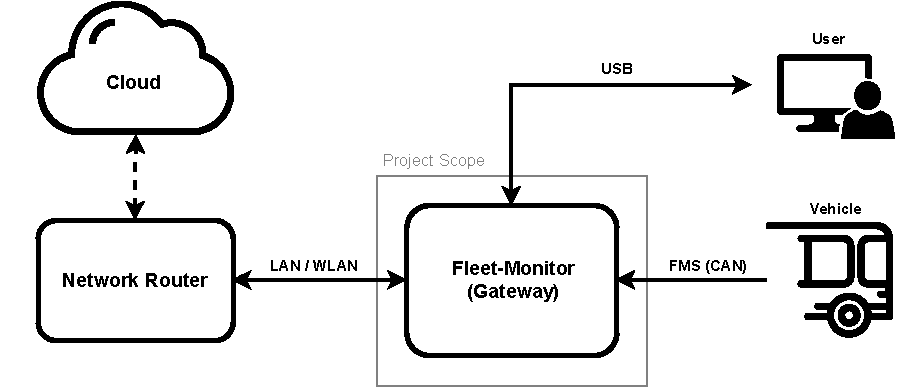
\includegraphics[width=\textwidth]{images/System_Overview}
	\vspace{-0.3cm}
	\caption{System Overview}
	\label{fig:system-overview}
\end{figure}

\section{Open Source}
From the beginning, it was decided that everything about the project would be released under an open source license. Both of us are huge supporters of open source and believe it will be the future of engineering. Building upon existing libraries and code under open source licences, allows us to accelerate the design process. Sometimes open source is considered an act of charity, but in our case, the benefits of using it outweigh any closed source processes. All documents and files of the project can be found on our GitHub page. A short description of all the repositories can be found in the Appendix \ref{Data Archive}.

\chapter{Requirements Specification and Project Schedule}

\theoremstyle{plain}
\theoremsymbol{}
\newtheorem{Rule}[theorem]{Rule}

\pagebreak
\section{Requirements Specification} \label{Requirements Specification}
\enlargethispage{2.5cm}
\begin{adjustwidth}{0.23cm}{0cm} \hfuzz=7.0pt
\makebox[\textwidth]{\frame{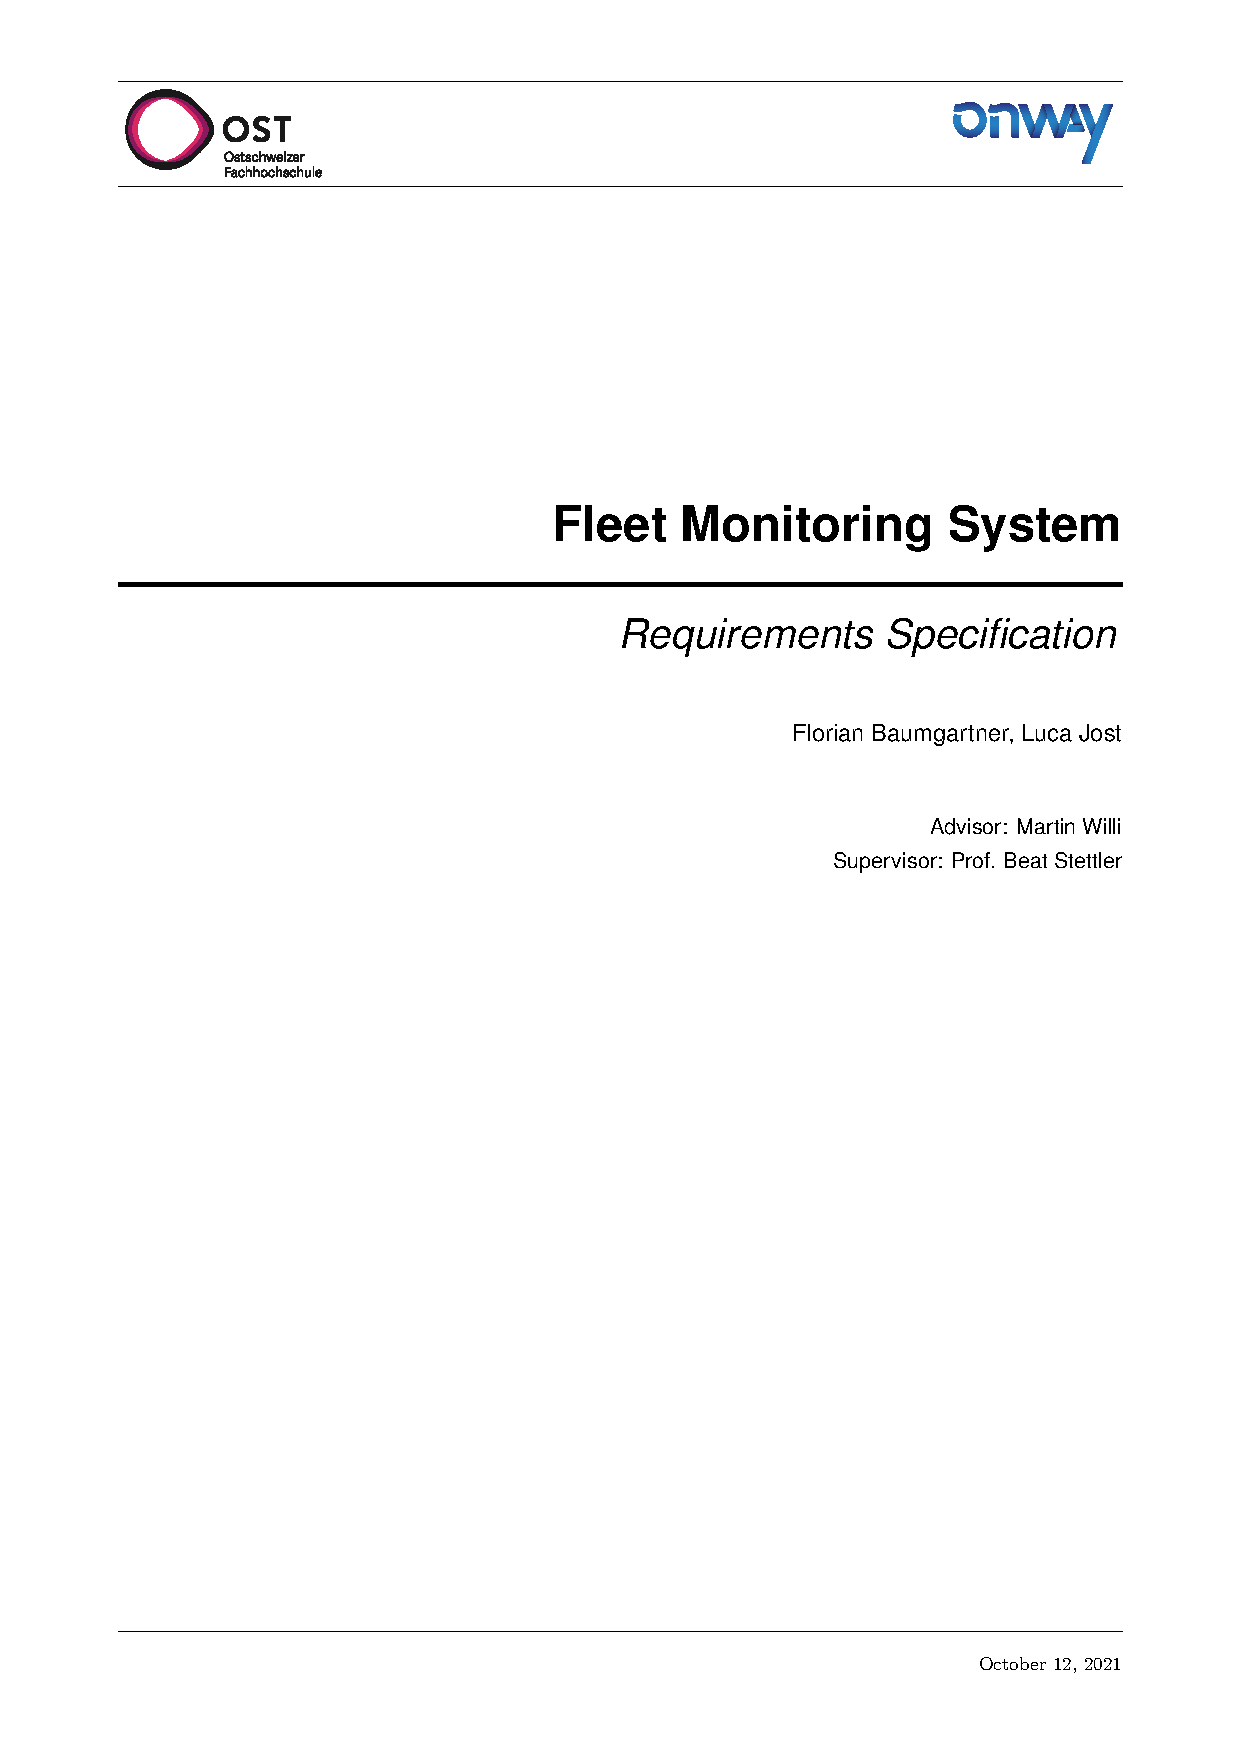
\includegraphics[width=17.3cm, page=1]{appendix/Requirements_Specification}}}
\end{adjustwidth}
\newpage

\begin{adjustwidth}{-0.23cm}{0cm} \hfuzz=7.0pt
\makebox[\textwidth]{\frame{\includegraphics[width=17.3cm, page=2]{appendix/Requirements_Specification}}}
\end{adjustwidth}
\newpage

\begin{adjustwidth}{0.23cm}{0cm} \hfuzz=7.0pt
\makebox[\textwidth]{\frame{\includegraphics[width=17.3cm, page=3]{appendix/Requirements_Specification}}}
\end{adjustwidth}
\newpage

\begin{adjustwidth}{-0.23cm}{0cm} \hfuzz=7.0pt
\makebox[\textwidth]{\frame{\includegraphics[width=17.3cm, page=4]{appendix/Requirements_Specification}}}
\end{adjustwidth}
\newpage

\begin{adjustwidth}{0.23cm}{0cm} \hfuzz=7.0pt
\makebox[\textwidth]{\frame{\includegraphics[width=17.3cm, page=5]{appendix/Requirements_Specification}}}
\end{adjustwidth}
\newpage

\begin{adjustwidth}{-0.23cm}{0cm} \hfuzz=7.0pt
\makebox[\textwidth]{\frame{\includegraphics[width=17.3cm, page=6]{appendix/Requirements_Specification}}}
\end{adjustwidth}
\newpage

\begin{adjustwidth}{0.23cm}{0cm} \hfuzz=7.0pt
\makebox[\textwidth]{\frame{\includegraphics[width=17.3cm, page=7]{appendix/Requirements_Specification}}}
\end{adjustwidth}
\newpage


\begin{landscape}
    \section{Project Schedule}
    \begin{figure}[h!]
    	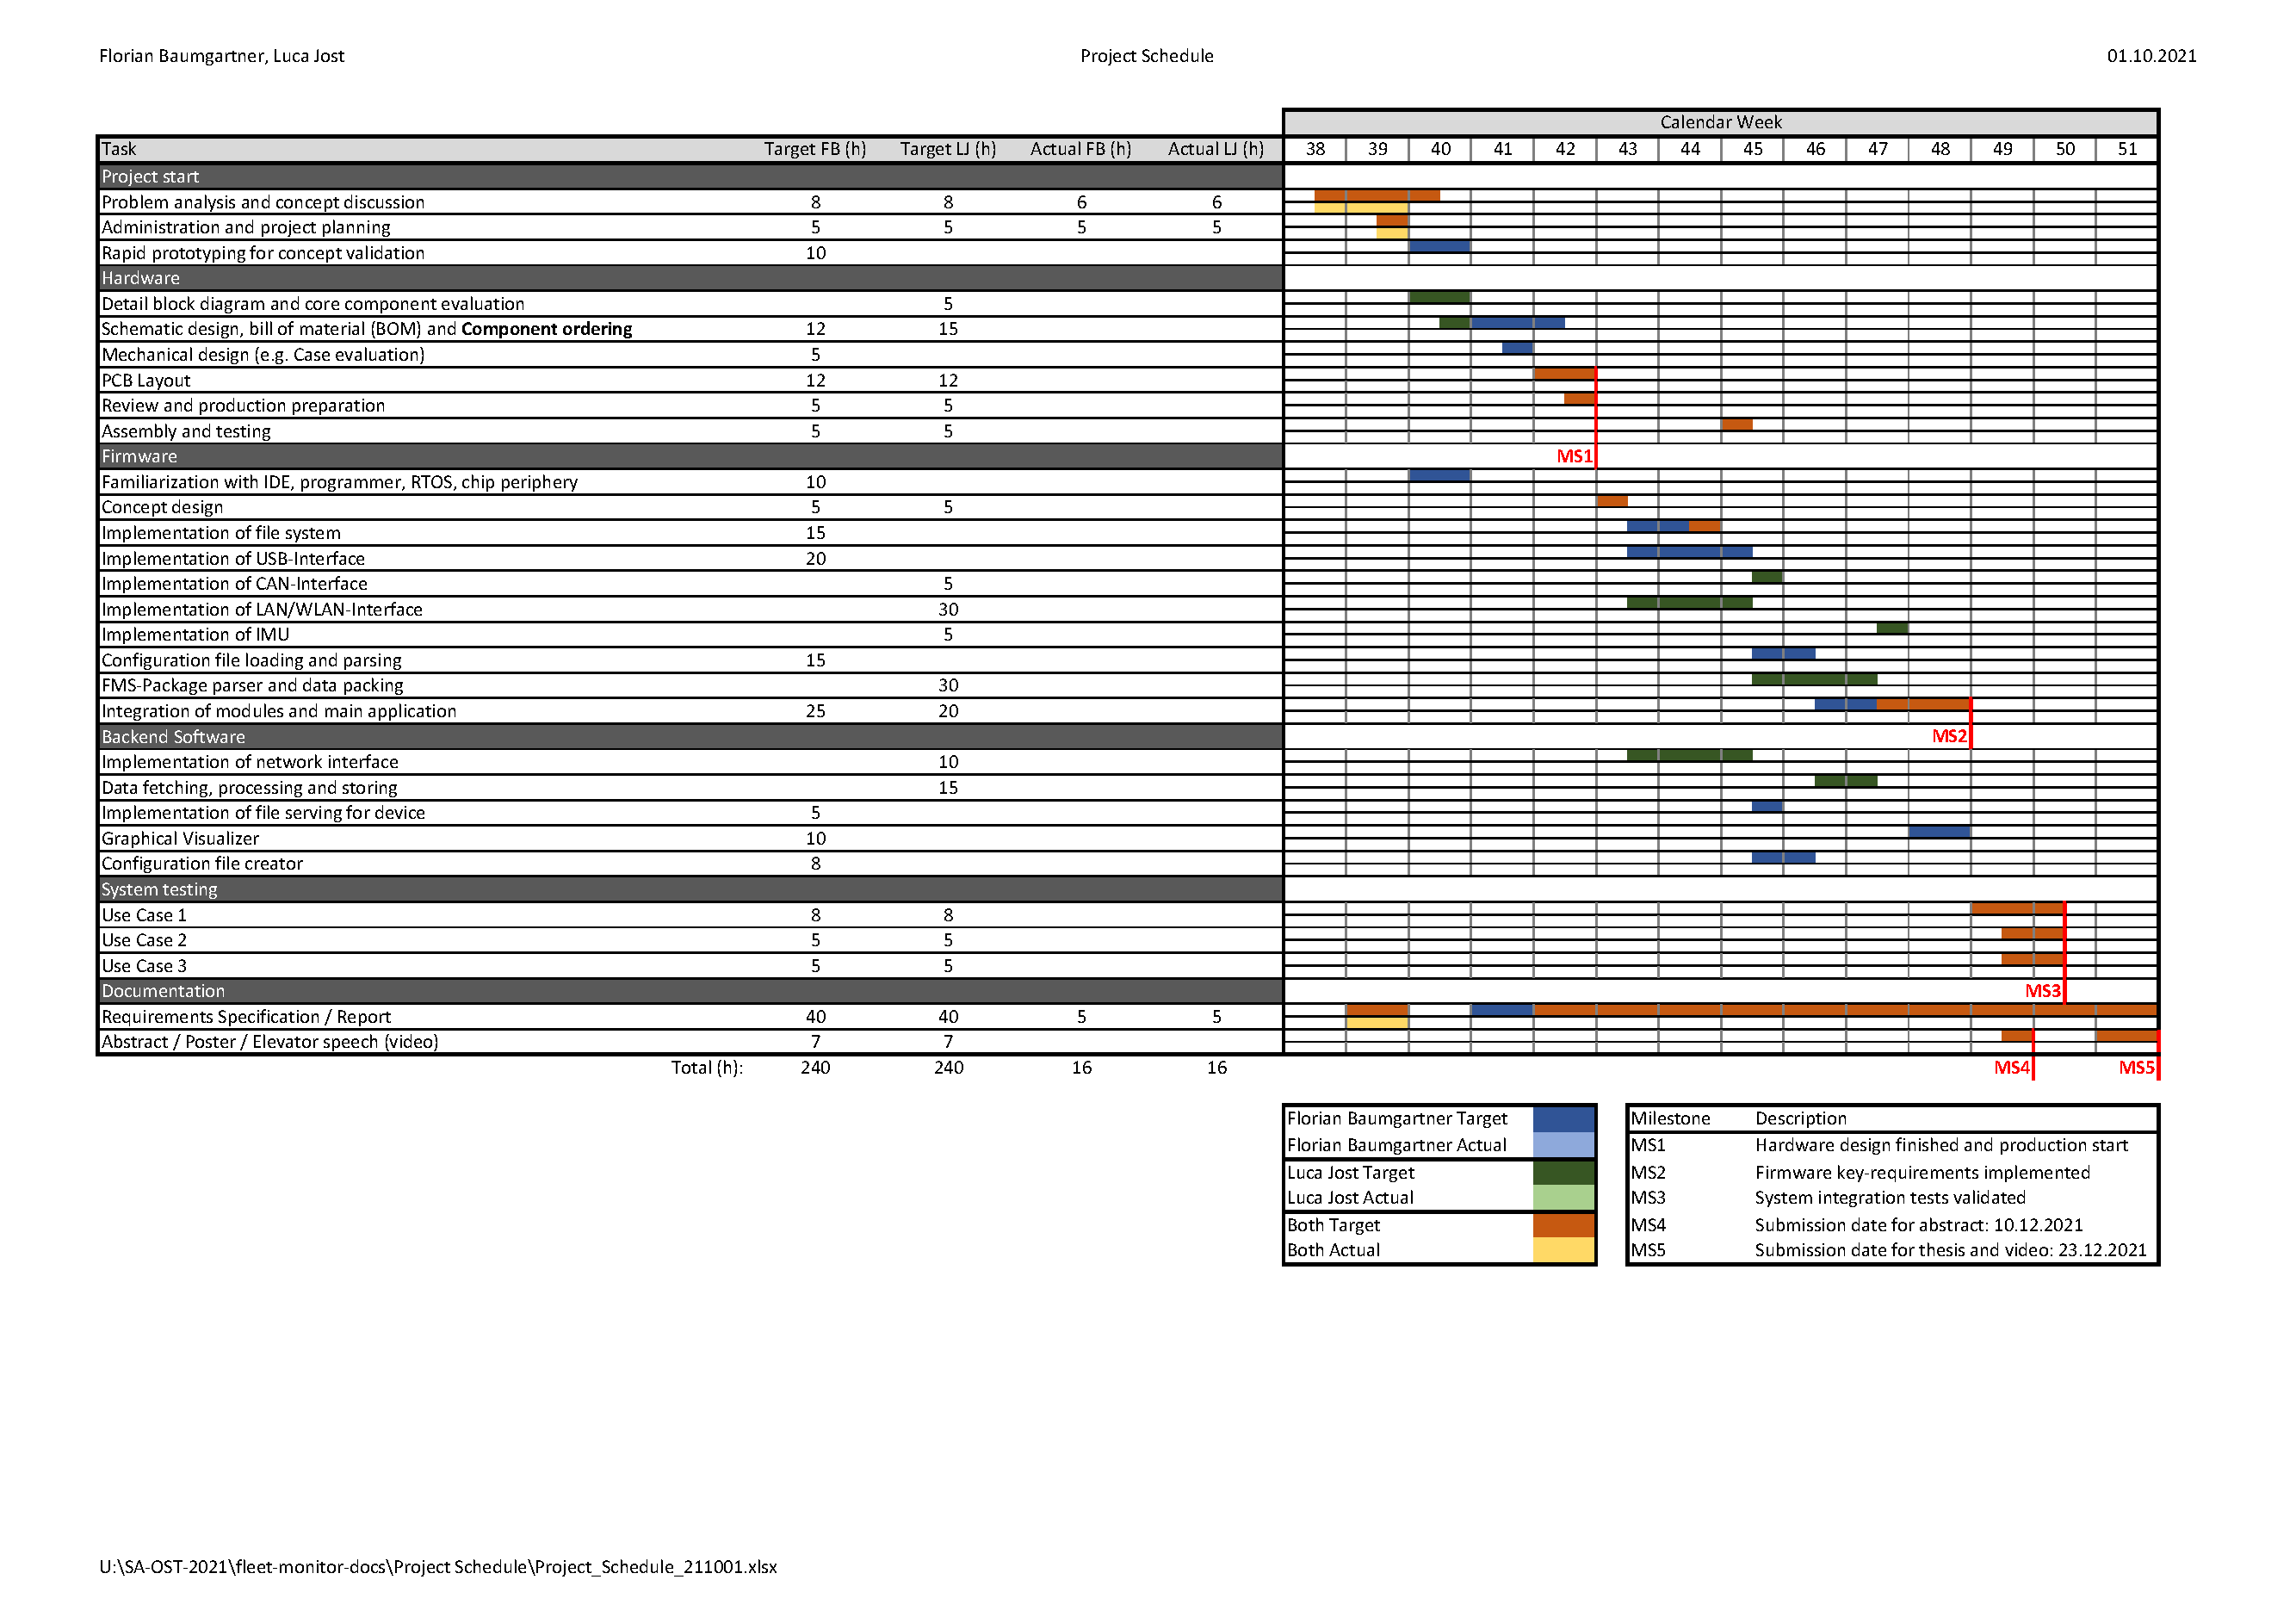
\includegraphics[height=13cm, trim=17mm 69mm 25mm 20mm, clip]{appendix/Project_Schedule_211001}
    	\bigskip
    	\caption{Project Schedule}
	    \vspace{-2cm}
	    \label{fig:project_schedule}
    \end{figure}
    \pagebreak

\end{landscape}
\chapter{Preliminaries}
\section{Controller Area Network (CAN)}
\subsection{Basics}
ISO11898 describes the physical data link layer implementation of \acrshort{can}. This specification describes a twisted-wire pair bus with 120 $\Omega$ line impedance, and differential signaling at a rate up to 1 Mbit/s. A network is constructed with two or more transceivers on the same bus lines. The network must be terminated with a 120 $\Omega$ resistor at each end of the bus, as shown in Figure \ref{fig:can-bus_topology}.

\begin{figure}[h!]
	\centering
	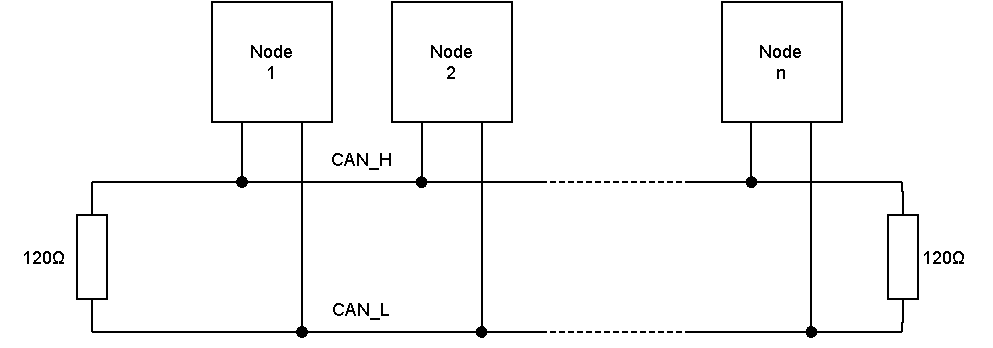
\includegraphics[height=3.8cm]{images/can-bus_topology}
	\caption{Topology of a \acrshort{can}-Bus}
	\label{fig:can-bus_topology}
\end{figure}

As long as the bus is free, any node is allowed to transmit \acrshort{can} messages. Each message is received by all nodes on the network, including the node that sent the message. This type of data broadcasting allows multiple nodes to use the transmitted data. It also allows the sending node to monitor the bus for errors. If two or more nodes try to transmit at the same time, the lower priority message will be overwritten, and this lower priority node will halt transmission upon sensing overwritten bits in its message identifier. The message is then re-transmitted when the bus is again free. This non-destructive process is called bit-wise arbitration.

Every node on the network reads the identifier of a message, and each node independently determines if the message is to be ignored or processed. Since the identifier is specific to the contents of the message rather than the identity of the originating node, new nodes may be added to the network, without modifying the program of any existing node on the network \cite{ti_can_transceivers}.
\newpage

\subsection{Signaling}
The signals on the CAN bus are distinguishes between two bus logic states, dominant and recessive. A recessive bit is defined as CANH being less than CANL + 0.5\,V. A dominant bit is defined as CANH being more than CANL + 0.9\,V. Figure\,\ref{fig:can-signaling} illustrates the nominal case. Since dominant bits overwrite recessive bits, CAN manages message collision through the process of bit-wise arbitration as described earlier.

\begin{figure}[h!]
	\centering
	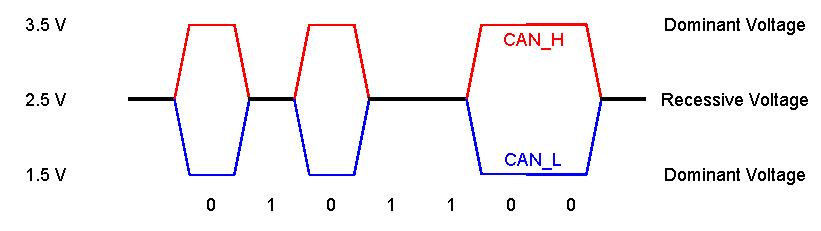
\includegraphics[height=3cm]{images/can-signaling}
	\caption{\acrshort{can}-Bus Signaling}
	\label{fig:can-signaling}
\end{figure}

\subsection{Frames}
Messages over a \acrshort{can} bus are referred to as frames. The most common frame types are defined as \acrshort{can} 2.0A and 2.0B also known as base and extended frame. 2.0A is simply a \acrshort{can} frame with an 11-bit identifier and 2.0B always uses 29-bit. A \acrshort{can} frame is always split up into the following regions \cite{can_bus_tutorial}.

\begin{figure}[h!]
	\centering
	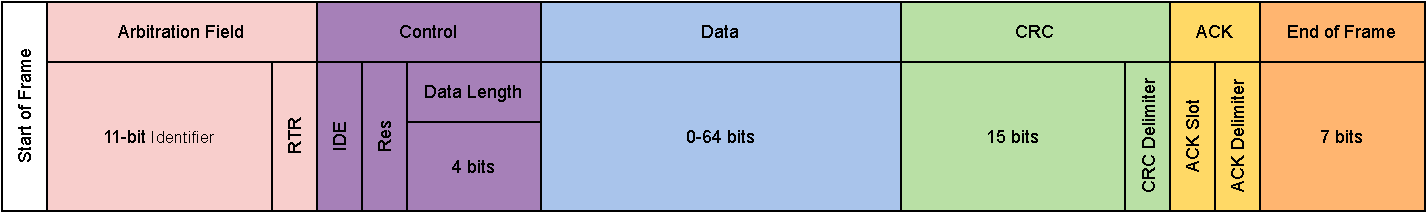
\includegraphics[height=2cm]{images/can-frame}
	\caption{Base 11-bit identifier \acrshort{can} frame}
	\label{fig:can-frame}
\end{figure}

\begin{itemize}
		\item The Arbitration Field, includes the identifier of the message and defines the priority. The identifier must be 11 or 29 bits long. Also in this field is the \acrfull{rtr} bit, which is used to request data.
		\item The Control Field is used to differentiate between the two frame types and defines the incoming data length.
		\item The data field can contain 0-8 bytes of information.
		\item The \acrshort{crc} field contains a 15-bit checksum. The checksum is used to detect errors in the transmission.
		\item The Acknowledgement Slot, is used to detect if a message was received by any of the devices on the bus. The transmitter checks for the presence of the Acknowledge bit and re-transmits the message if no acknowledge was detected.
\end{itemize}
\newpage

\section{SAE J1939}
J1939 is the open standard developed by \acrfull{sae}. It is used for networking and communication in the commercial vehicle sector. J1939 is a higher-layer protocol utilizing \acrshort{can} as its physical layer. SAE J1939 is primarily a data driven protocol, providing far better data bandwidth than other automation protocols such as \gls{canopen} and \gls{devicenet} \cite{introduction_sae_j1939_protocol}.

The standard specifies CAN bus speeds of 250\,kbit/s or 500\,kbit/s and uses the extended 29-bit identifier frame format. Most messages defined by the J1939 standard are intended to be broadcast only. This means that the data is transmitted on the network without a specific destination. This permits any device to use the data without requiring additional request messages. The 29-bit identifier used in J1939 is structured in the following way \cite{sae_j1939_introduction}. 

\begin{figure}[h!]
	\centering
	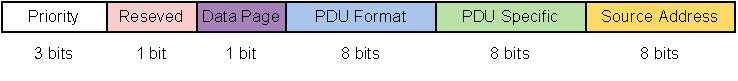
\includegraphics[height=1.5cm]{images/j1939-identifier}
	\caption{29-bit J1939 Identifier}
	\label{fig:29-bit_J1939_Identifier}
\end{figure}

The first three bits of the identifier are used for controlling a message priority during the arbitration process. A value of 0 has the highest priority.

The Reserved bit, Data Page bit, PDU Format field and PDU specific field are often grouped together and referred as \acrfull{pgn}. 

The last 8 bits of the identifier contain the address of the device transmitting the message. Two devices can not share the same address.
\newpage

\section{Fleet Management System (FMS)}
The Fleet Management Systems Interface (FMS) is a standard interface developed by European commercial vehicle manufacturers in 2002. It defines a common interface for telematics applications and include driving as well as diagnostics information. The data is coded according to the SAE J1939 standard. FMS is a broadcast only system, a gateway between the internal bus and the FMS bus is implemented by the OEM. 3rd party systems, like the Fleet-Monitor, are forbidden on the internal bus as shown in figure \ref{fig:fms-bus}. 

\begin{figure}[h!]
	\centering
	\hfuzz=14.0pt
	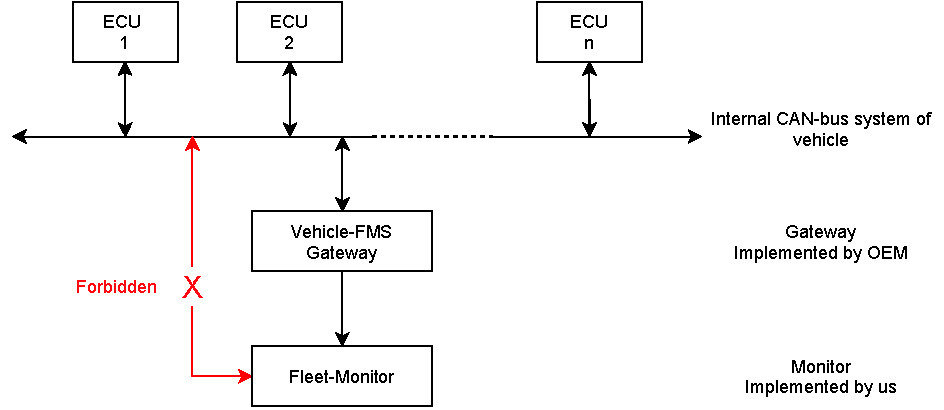
\includegraphics[height=6.5cm]{images/fms-bus}
	\caption{FMS Topology}
	\label{fig:fms-bus}
\end{figure}

At the time of writing, the standard includes 36 different packages, ranging from engine coolant temperature to door position.  Depending on the frame, updates occur between 20ms and 10s. The convention set the \acrfull{pgn} for J1939 identifiers, while the OEM specify the source address and priority. Each frame has a fixed data length of 8 byte but not all of them contain information. Example of a FMS Frame:

\begin{figure}[h!]
	\centering
	\hfuzz=11.0pt
	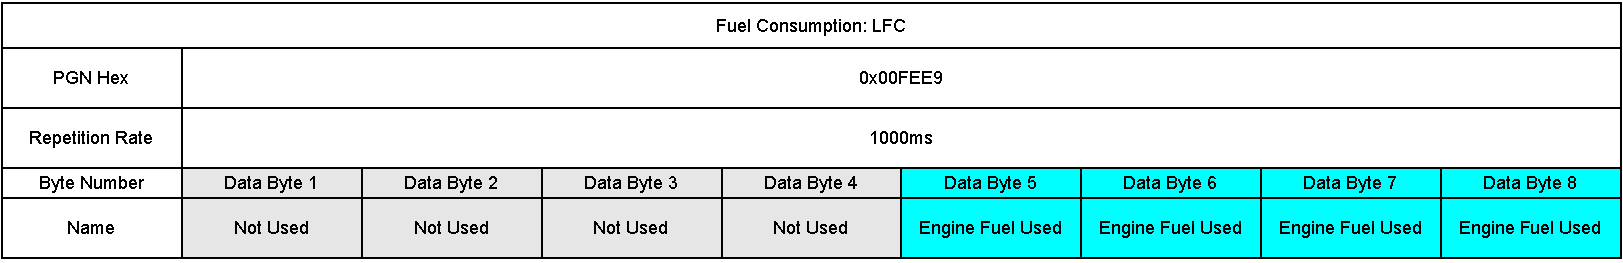
\includegraphics[height=2.4cm]{images/fms-frame}
	\caption{Fuel Consumption FMS Frame}
	\label{fig:fms-frame}
\end{figure}


\chapter{Development}

\section{Hardware Design}
The hardware of the Fleet-Monitor was design using Altium Designer 21. The integrated 3D \acrshort{cad} functionality simplified the overall development and lowered the chance of errors in the design. The 4-Layer \acrfull{pcb} with the size of 140.5 mm x 79.5 mm has been manufactured and assembled by JLCPCB.\newline
As a proof of concept, five prototypes have been made, which are all fully tested and in working condition.

\todo{Add Rendering of PCB only}
\medskip
\begin{figure}[h!]
	\centering
	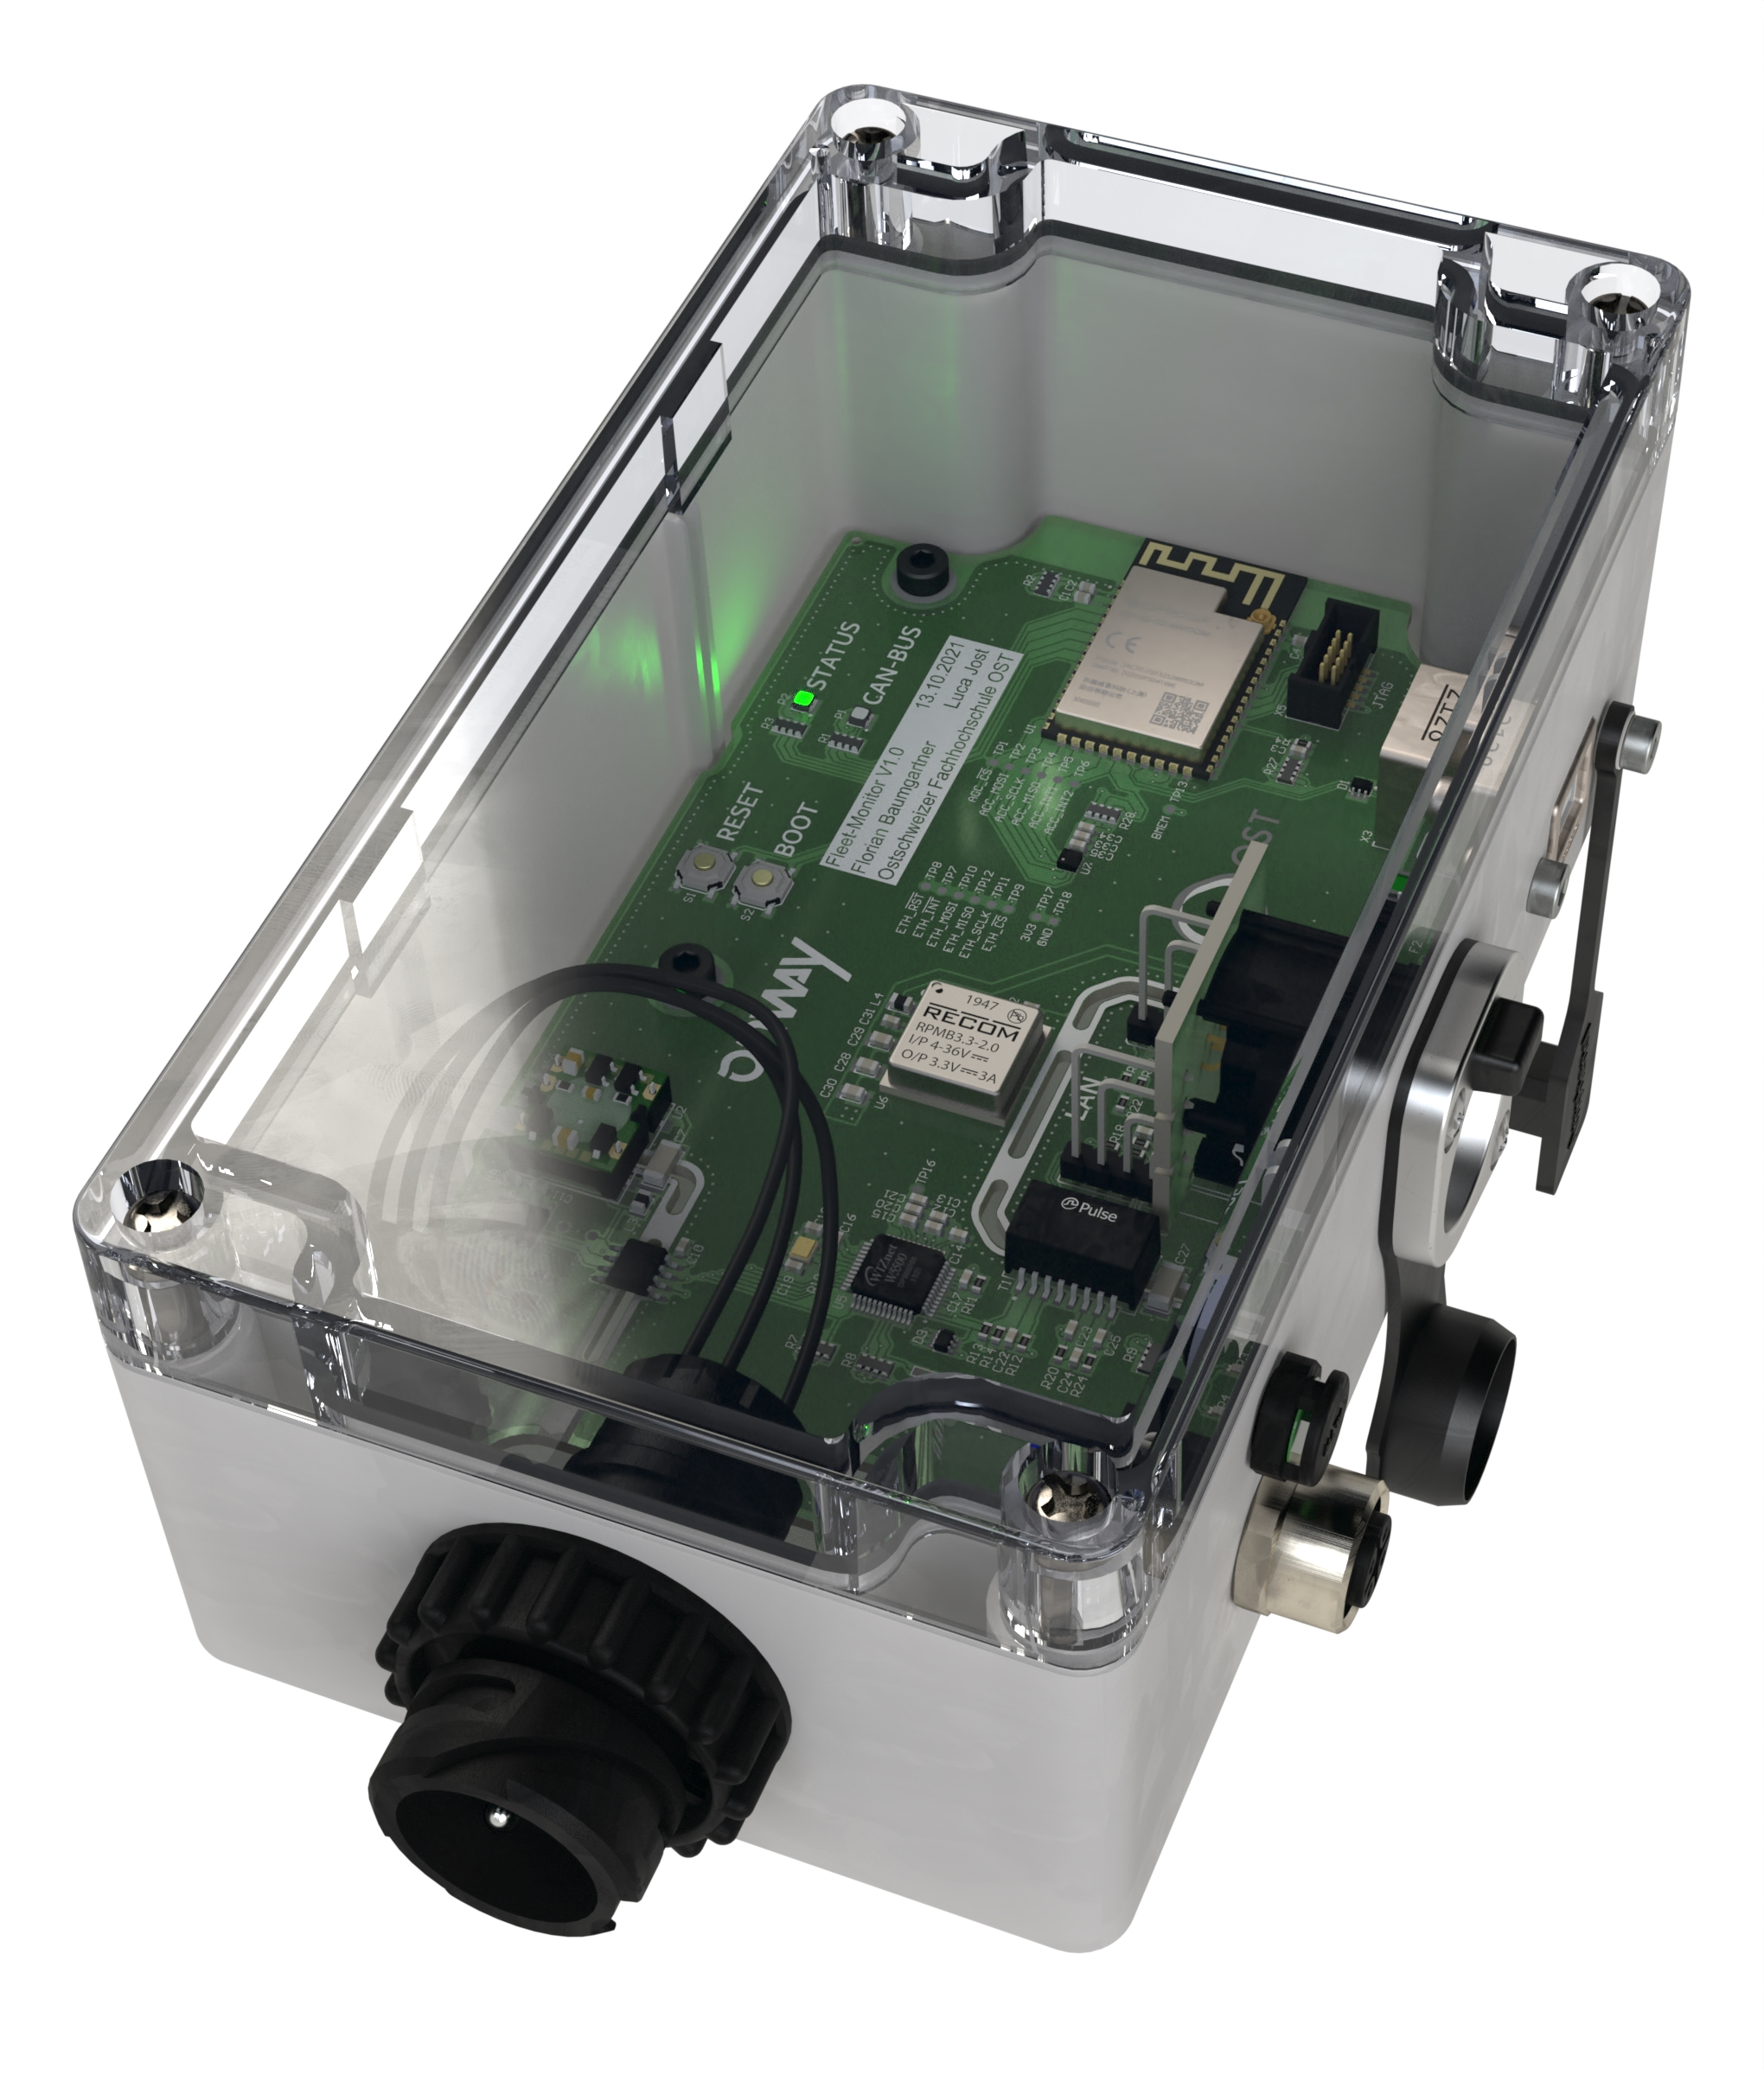
\includegraphics[height=9cm]{images/fleet-monitor-rendering}
	\caption{Assembled PCB 3D-Render}
	\label{fig:fleet-monitor-rendering}
\end{figure}

\subsection{Power Management}
The device can be powered ether by the \acrshort{usb}-Interface or an external DC power source. Both supply options are internally connected through Schottky diodes and provide a seamless switch-over. If both supply sources provide power at the same time, the external one gets preferred.\newline
The \acrfull{usb} Interface fulfills all guidelines of the \acrshort{usb} specifications in terms of power consumption. Therefor it is guaranteed, that the maximal current of 500 mA is not exceeded. In case of failure, a resettable \acrshort{ptc} Poly-fuse protects the power source of potential over current.\newline
The external power source accepts a voltage range from 9 V to 28 V and is protected against wrong polarization and short circuit. As a suitable connector, the industry standard M12 (5 Pin) type has been chosen. It fulfils the IP67 rating and is highly robust against accidental disconnection due to its threaded coupling. In addition it is used in a wide variety of applications, resulting in great availability. The pin-out consists of pin 1 and 2 used for the positive input and pins 3 to 5 for ground. This has the advantage, that matching connectors with a different amount of pins (e.g. 2-pin connector) can be used as well.\newline
The core of the power management unit is based on a Recom DC-DC converter of the RPMB-2.0 series. The very compact design, great performance and fairly low price offers an optimal solution.\newline
The total power consumption of the device is in average around 1.5 W.

\todo{Add PTC Fuse in fron of diode in diagram}
\begin{figure}[h!]
	\centering
	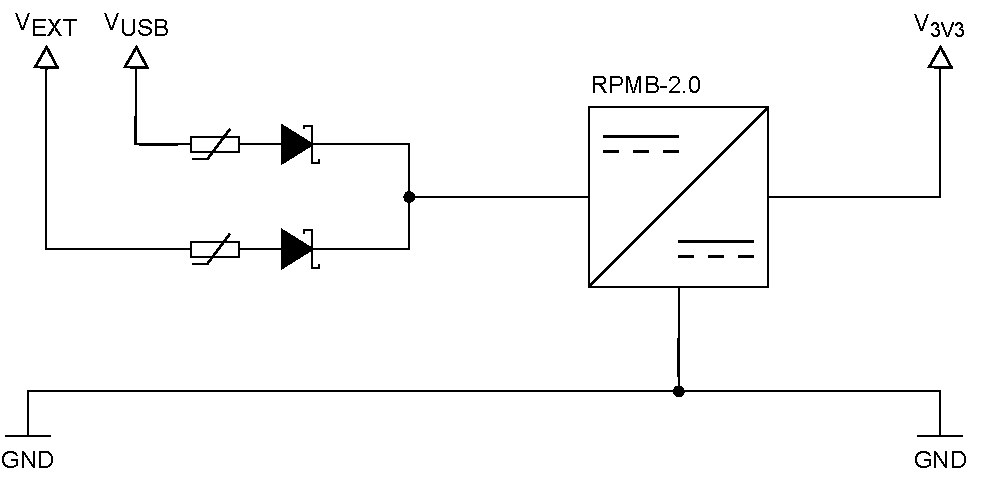
\includegraphics[height=5cm]{images/power}
	\caption{Simplified Power Management}
	\vspace{-1.4ex}
	\label{fig:simplified-power}
\end{figure}
\newpage

\subsection{ESP32-S2}
The choice of a suitable micro controller is crucial in the design of an embedded system. Several factors were carefully considered and key requirements have been set, such as:

\begin{itemize}
		\item Integrated Wi-Fi subsystem and \acrshort{rf} front-end
		\item System performance: CPU speed, memory and peripherals
		\item Native \acrshort{usb} 2.0 Interface
		\item Physical package and pin count
		\item Availability (especially in an ongoing worldwide chip-shortage)
\end{itemize}

The Espressif's \gls{esp32} \acrfull{soc} family satisfies all listed requirements and is in addition advertised as a low cost solution.\newline
To reduce design complexity and production cost, the ESP32-S2 has been embedded as a solder-on module of the type ESP32-S2-WROOM-I. This module has the advantage of containing the RF front-end inclusive an integrated \acrshort{pcb} antenna as well as a 4 MB \acrshort{spi} flash chip.\newline

%\medskip
\begin{figure}[h!]
	\centering
	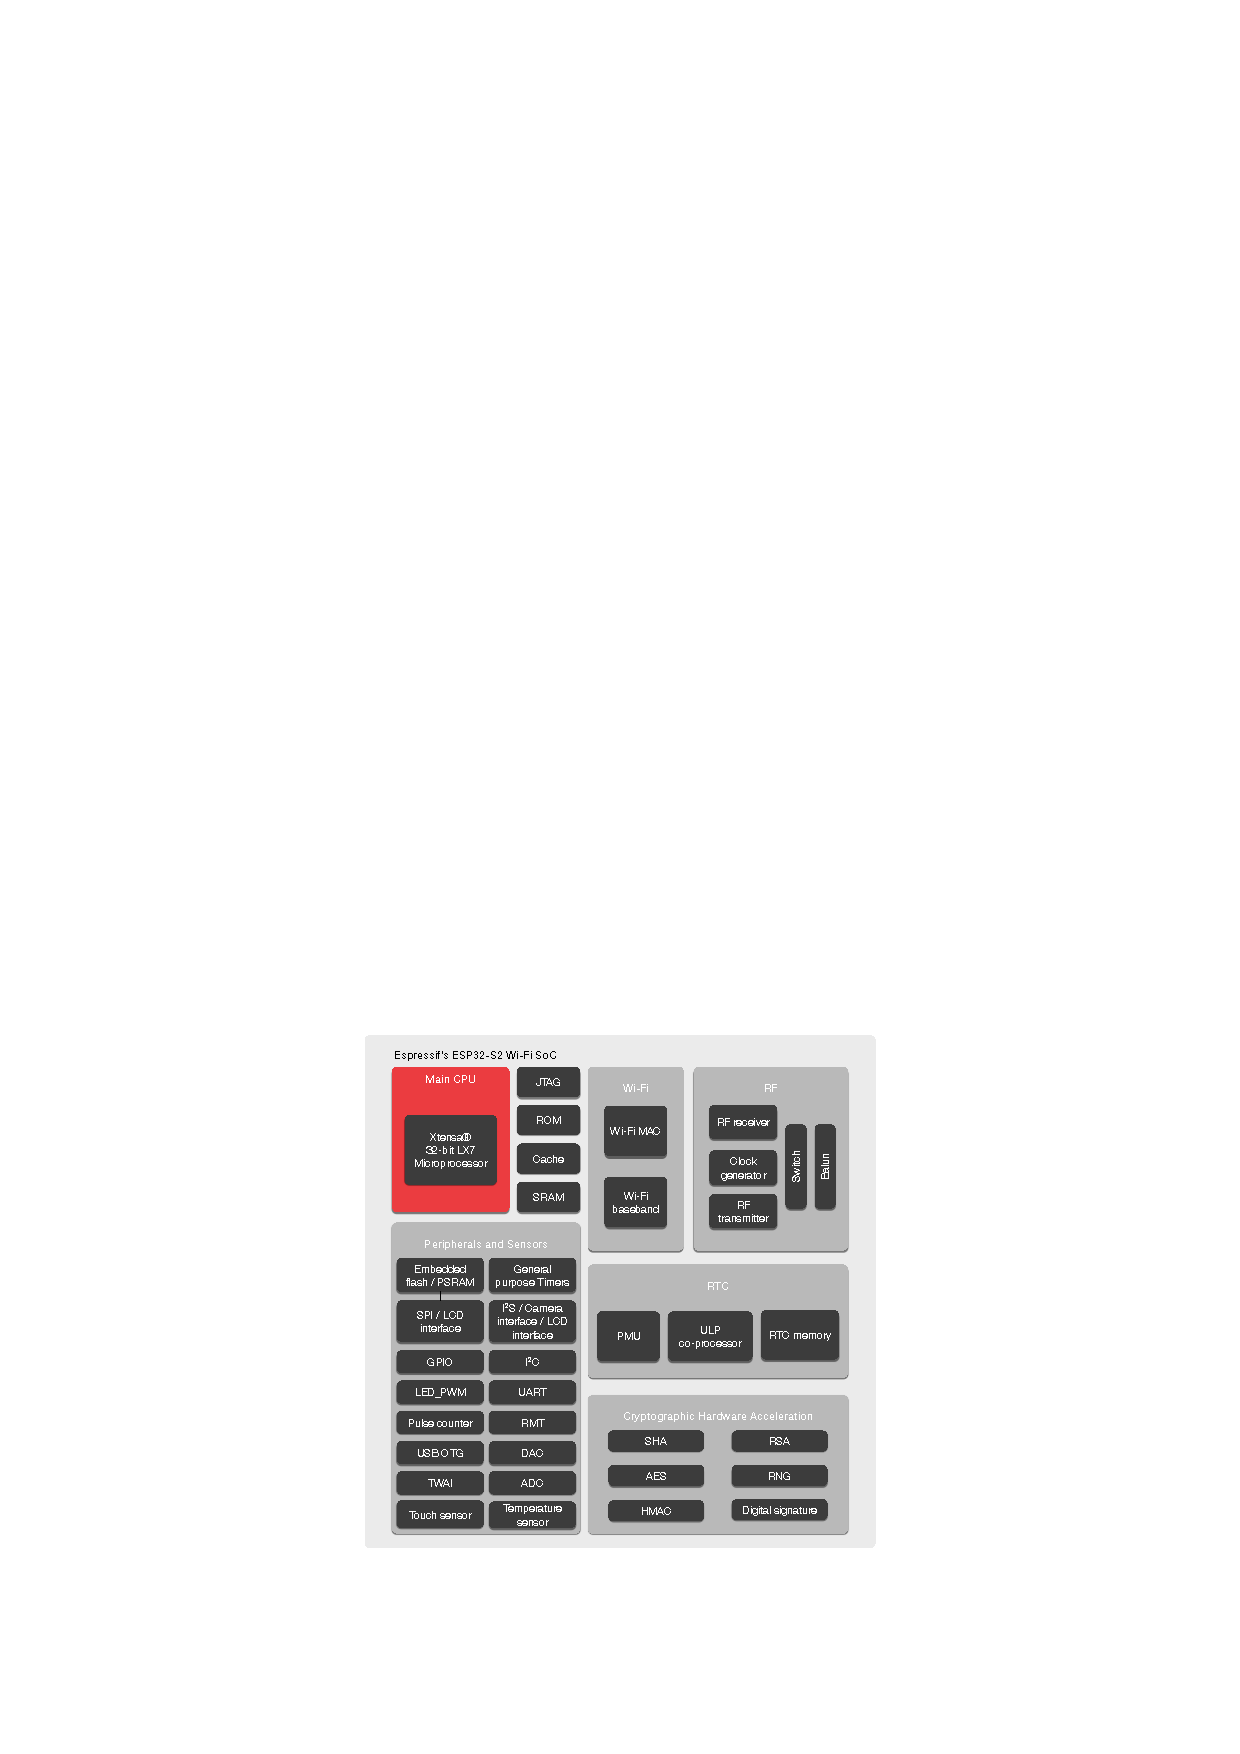
\includegraphics[height=9cm]{images/esp32-s2_block_diagram}
	\caption{ESP32-S2 Block Diagram}
	\vspace{-1.4ex}
	\caption*{\textbf{Source:} ESP32-S2 Datasheet \cite{esp32-s2_datasheet}}
	\label{fig:esp32-s2_block_diagram}
\end{figure}

The \acrshort{soc} can be programmed ether by \acrshort{jtag} and a suitable programmer (e.g. Espressif's ESP32-Prog) or conveniently over the integrated \acrshort{usb}-Interface.\newline
For uploading code via the \acrshort{usb}-Interface, the ESP32-S2 has to be set in to the device firmware update mode. This can be achieved by pressing the boot button while the device is booting (e.g. after powering on or a reset). If the boot button is not accessible, the user can force the device to enter the \acrshort{dfu} mode by setting a flag in the system configuration. This procedure gets further explained in the user manual section.\newline
\newpage

\subsection{Ethernet Interface}
The Ethernet interface utilizes a WIZNet W5500 Ethernet controller chip with an integrated \acrshort{phy} and \acrshort{tcp/ip} stack. It is capable of transmission speeds of 10 or 100 MBit/s. The chip is connected through \acrshort{spi} with the main processing unit (\gls{esp32}).
The IEEE standard 802.3 specifies a 1500 V\textsubscript{RMS} isolation barrier between the Ethernet PHY Chip and the cable. To comply with these requirements a pulse transformer was used to magnetically couple the data lines between the connector and the chip. Additionally a ground clearance of \todo{add distance} mm was chosen to avoid flash over or tracking between electrical conductors as seen in \todo{add image}. 

\begin{figure}[h!]
	\centering
	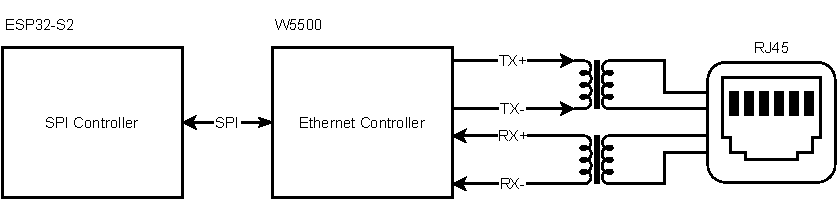
\includegraphics[height=2.5cm]{images/eth_interface}
	\caption{Simplified Ethernet Interface}
	\vspace{-1.4ex}
	\label{fig:eth-interface}
\end{figure}

\todo[inline]{Write about Ethercon ® connector}

\begin{figure}[h!]
	\centering
	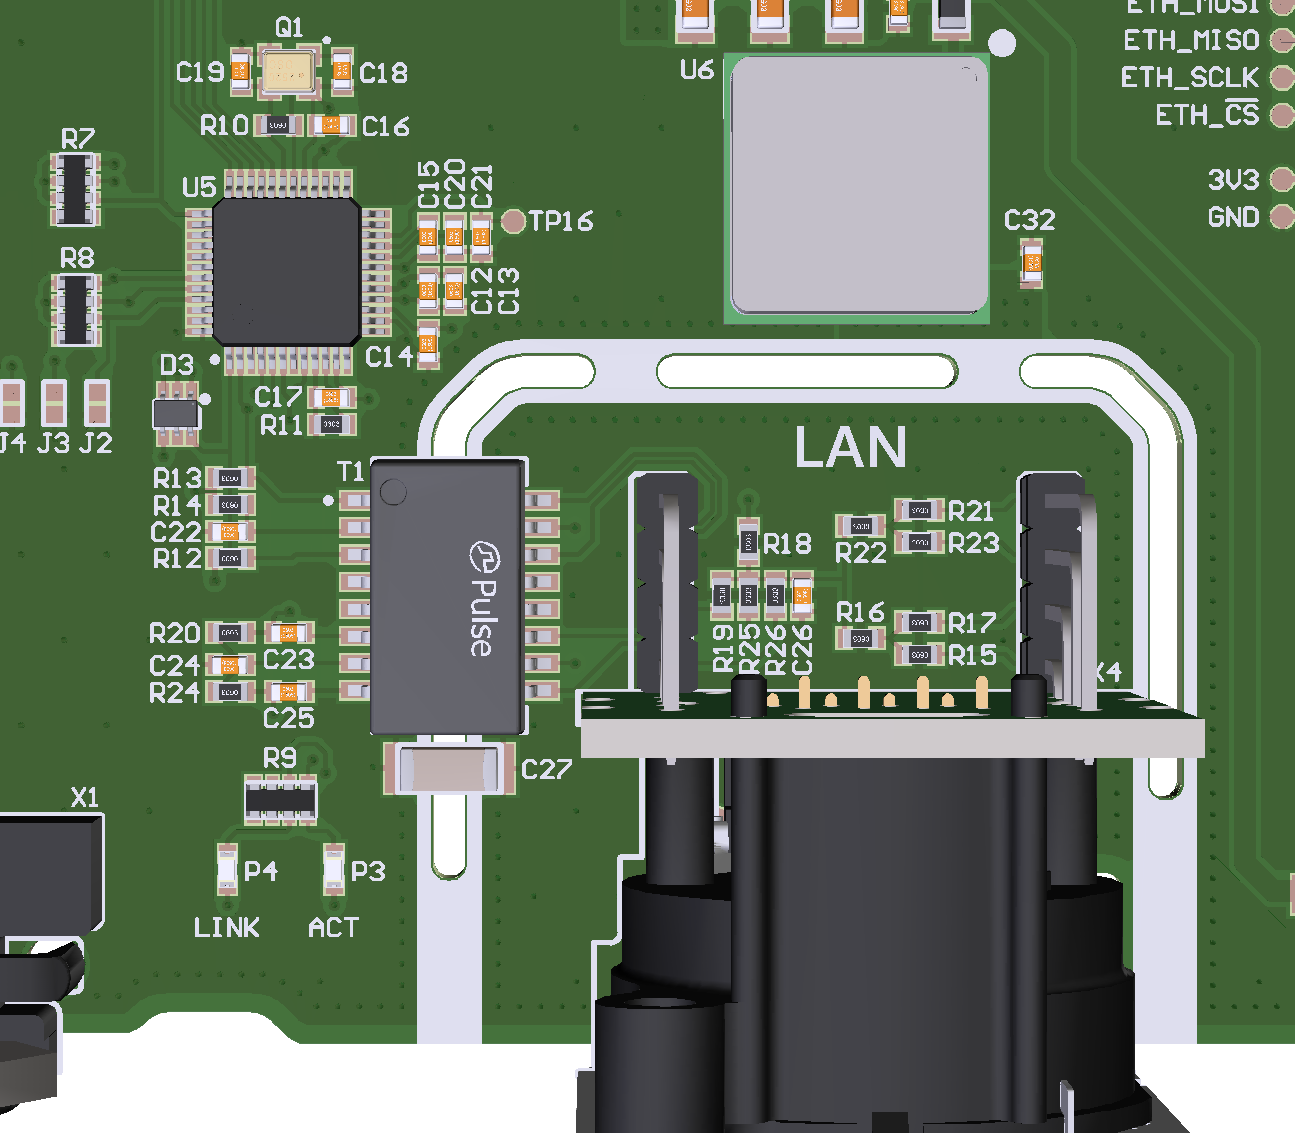
\includegraphics[height=7cm]{images/eth-pcb}
	\caption{PCB view of Ethernet Interface}
	\vspace{-1.4ex}
	\label{fig:eth-pcb}
\end{figure}

\newpage

\subsection{CAN-Bus Interface}
The \acrfull{twai} is a real-time serial communication protocol suited for automotive and industrial applications. It is compatible with CAN bus frames following the ISO11898-1 standard. The ESP32-S2 contains a \acrshort{twai} controller that can be configured to communicate on a CAN bus via an external transceiver.

\begin{figure}[h!]
	\centering
	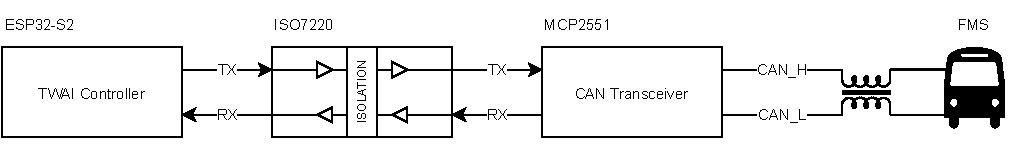
\includegraphics[height=1.8cm]{images/can-interface}
	\caption{Simplified CAN Interface}
	\vspace{-1.4ex}
	\label{fig:can-interface}
\end{figure}

\subsubsection{Transceiver}
The data lines are translated using a CAN transceiver from Microchip (MCP2551). The role of the transceiver is to drive and detect data to and from the bus. It converts the single-ended logic used by the controller to the differential signal transmitted over the bus. The MCP2551 device provides transmit and receive capabilities and is fully compatible with the ISO-11898 standard. \newline

\subsubsection{Isolation}
A dual-channel digital isolator (ISO7221BDR) was used in conjunction with an isolated DC/DC converter from Recom (R1SX-3.305/H). These devices block high voltage and isolate grounds, as well as prevent noise currents on a data bus or other circuits from entering the local ground and interfering with or damaging sensitive circuitry.

\begin{figure}[h!]
	\centering
	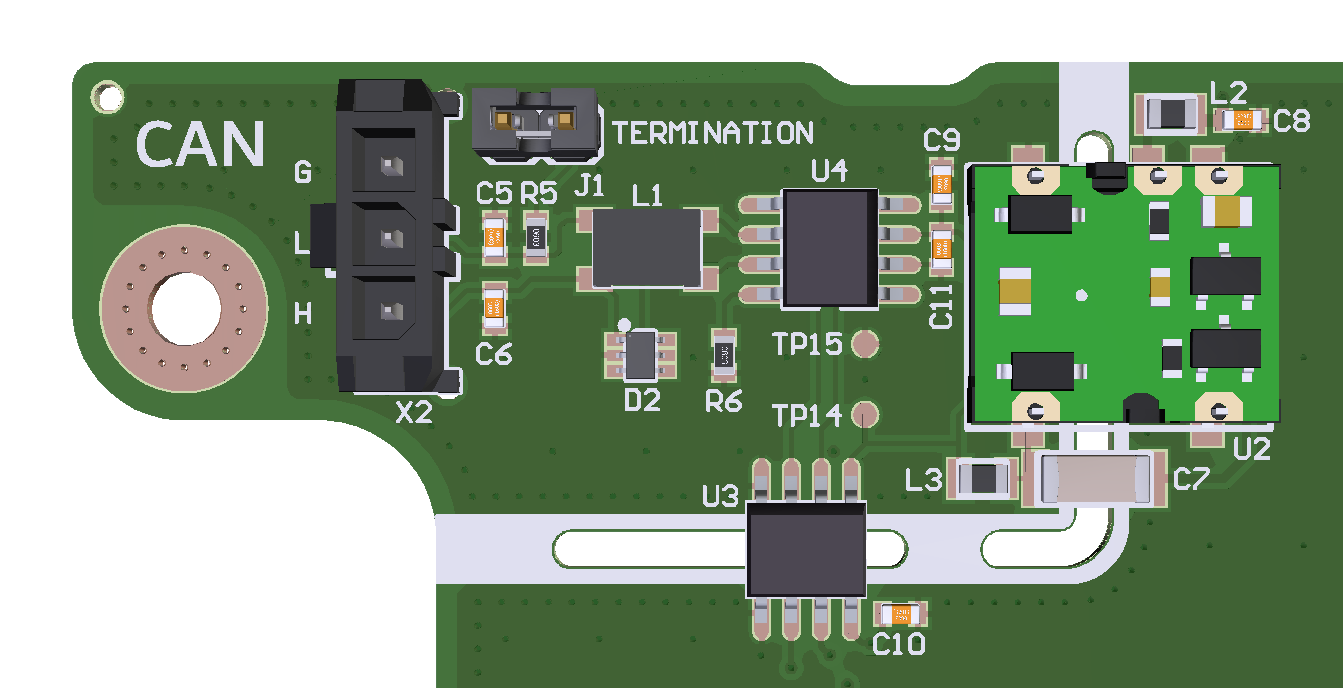
\includegraphics[height=4.5cm]{images/can-pcb}
	\caption{PCB view of CAN interface}
	\vspace{-1.4ex}
	\label{fig:can-pcb}
\end{figure}

\subsubsection{Filter}
A common mode choke as well as bypass capacitors were added to the differential signal lines. A common mode choke is an electrical filter that blocks high frequency noise common to two or more data or power lines while allowing the desired DC or low-frequency signal to pass. Common mode (CM) noise is typically radiated from sources such as radio signals, unshielded electronics, inverters and motors. Additionally matching capacitors on the CANH and CANL lines were added to enhance the immunity against electromagnetic interference. 

\subsubsection{Connector}
The FMS Standard specifies a DIN 72585 connector as the default physical interface. Since these connectors are only available for panel mount, an additional wire to board connector was selected. A Molex \todo{connector name} was chosen because its widely available and being used in lots of applications.\newline

\subsubsection{Termination}
In addition the FMS Standard specifies a 120$\Omega$ CAN termination resistor to be added on the monitor side. To fulfill this requirement and to make it compatible with system that do not need that resistor, a jumper was added to enable/disable the termination.   
\subsection{Accelerometer}
Luca

\newpage
\section{Mechanical Design}
The automotive environment is known for its harsh conditions, such as vibrations, large temperature range and high humidity. The device must withstand those factors and should guarantee a long lifespan. The optimal selection of components, especially the connectors was key to satisfy the requirements and reach an IP67 rating.\newline
As a suitable case for the device, a poly-carbonate watertight enclosure with transparent lid has been chosen. The very robust construction creates an ideal protection for all electronic components.\newline
The case has been machined in the internal workshop of the university. The corresponding mechanical drawings have been made with SolidWorks 2020 and are attached in the appendix: \ref{Fleet-Monitor V1.0 Mechanical Drawing}

\medskip
\begin{figure}[h!]
	\centering
	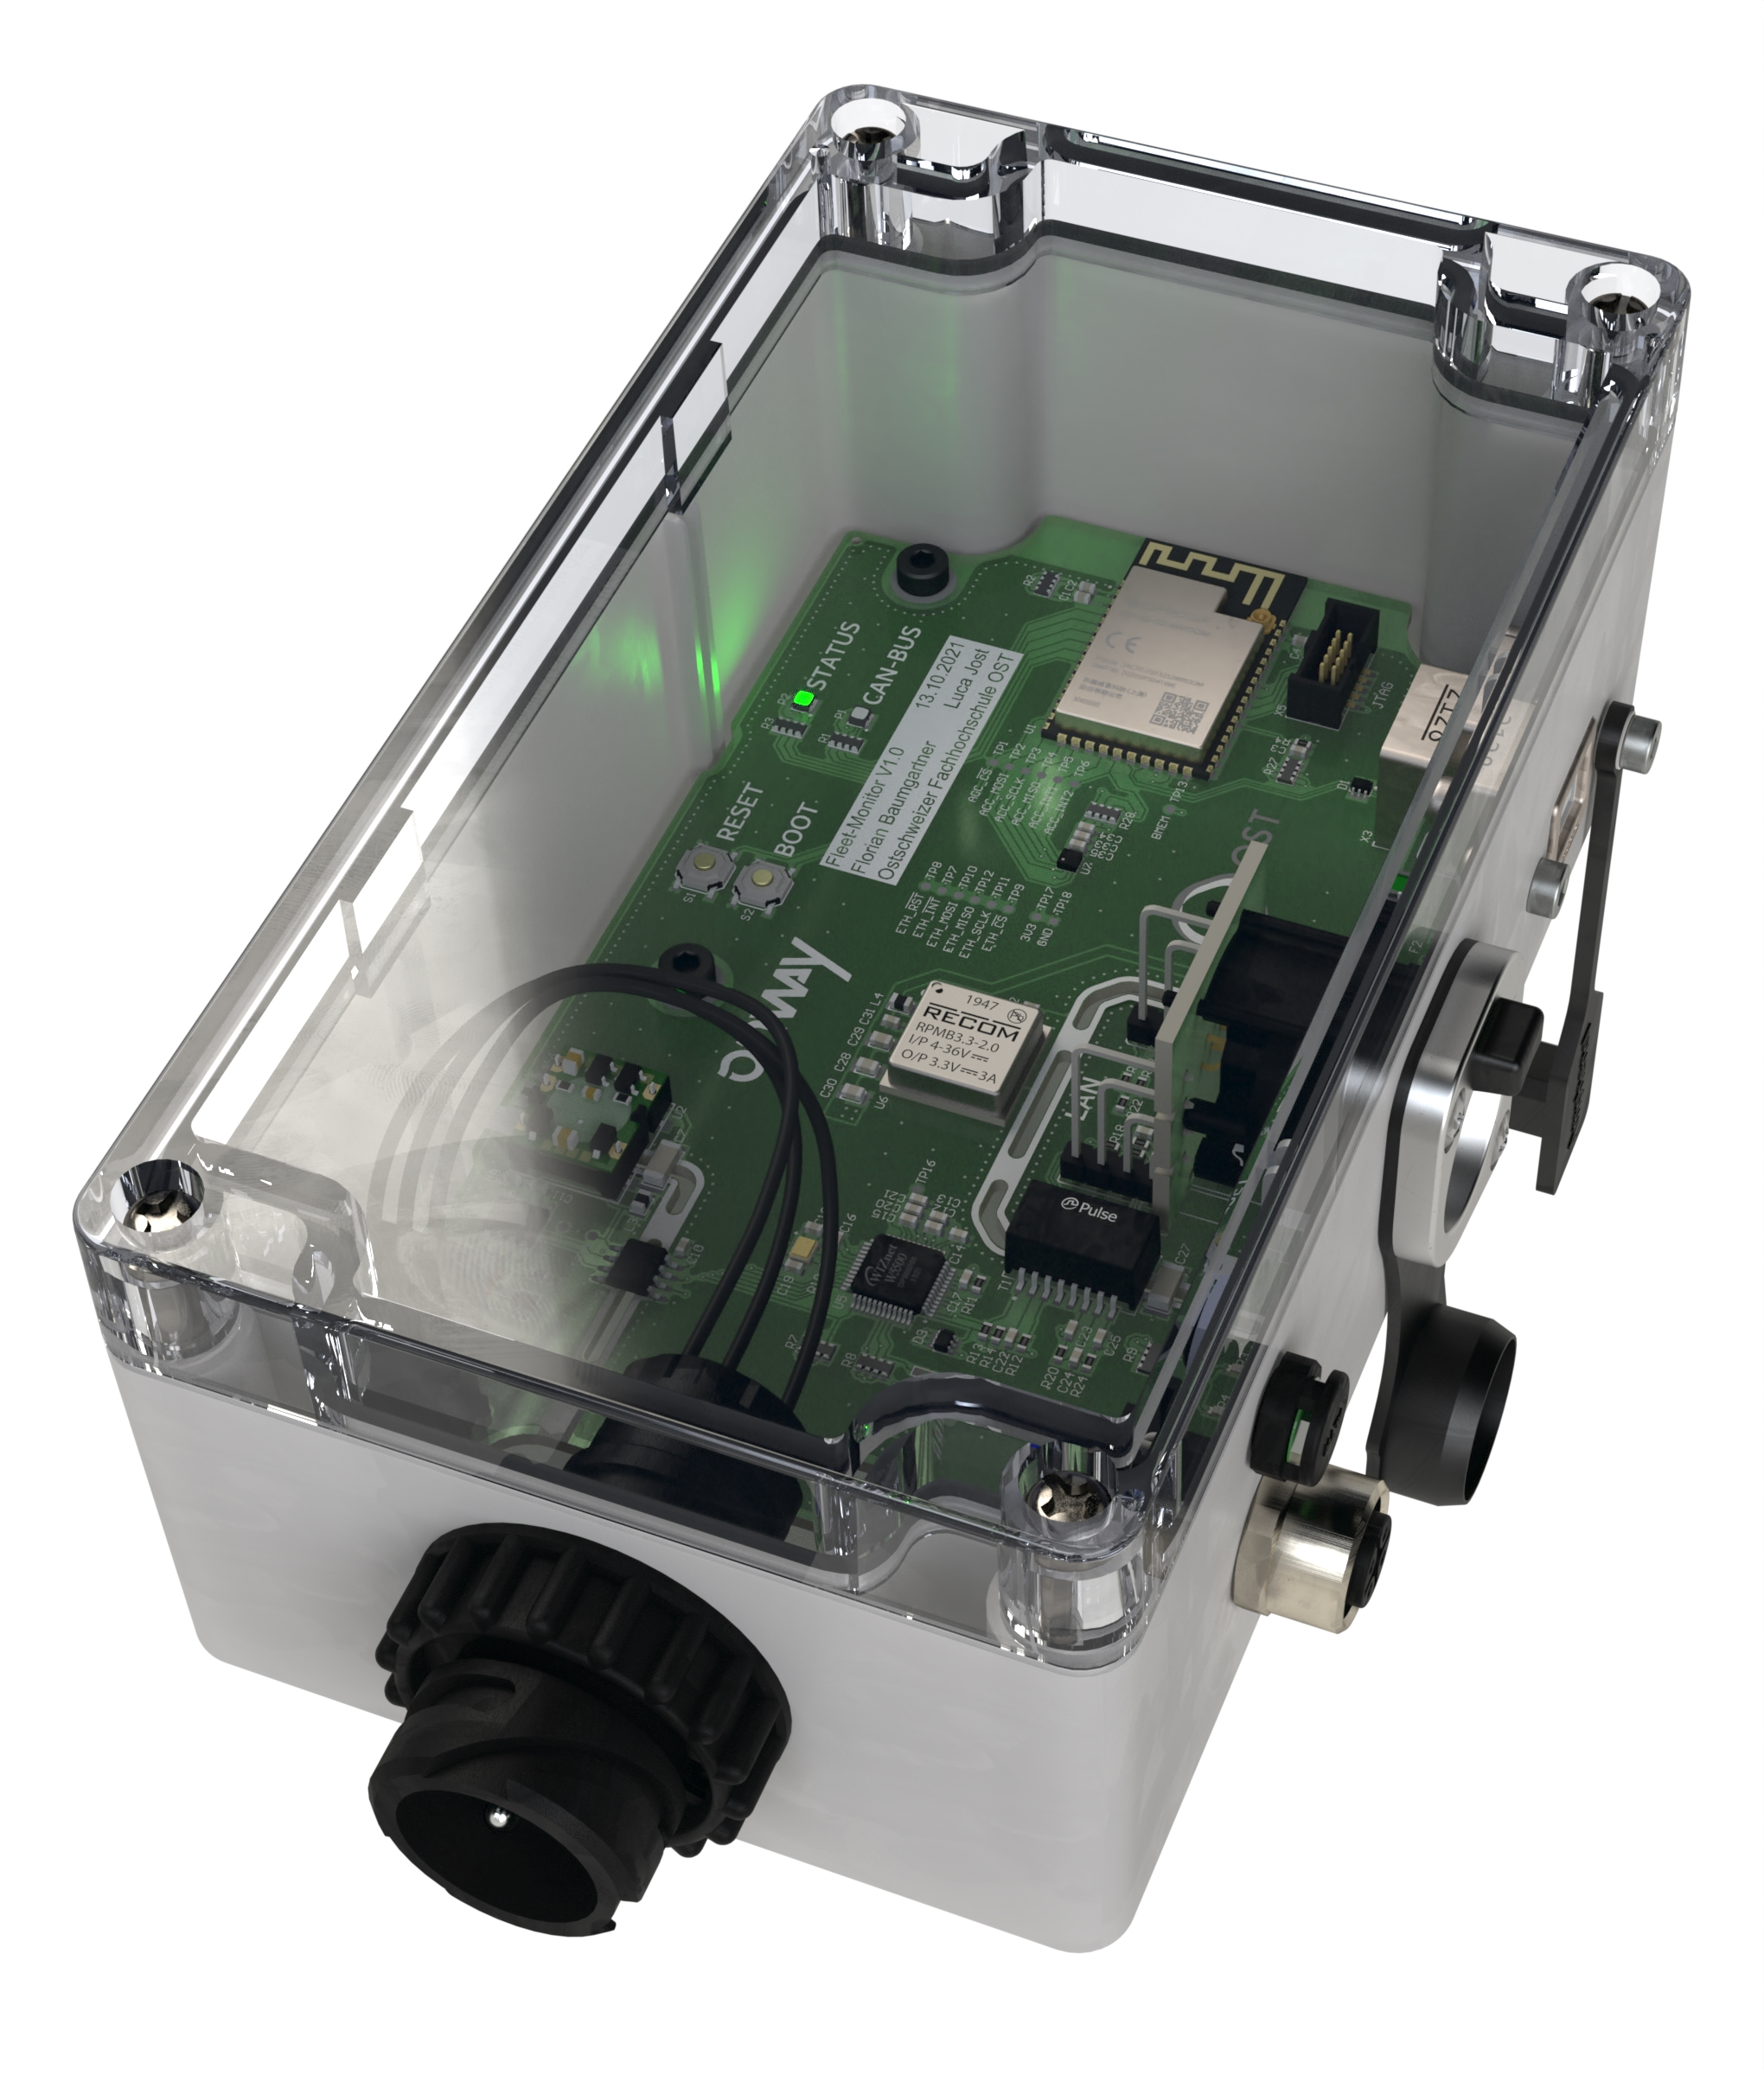
\includegraphics[height=16cm]{images/fleet-monitor-rendering}
	\caption{Final Product 3D-Render}
	\label{fig:fleet-monitor-rendering}
\end{figure}


\newpage
\section{Firmware}
The firmware is written in C++ and is based on a combination of the Arduino and the ESP-IDF framework. As an IDE, Visual Studio Code with PlatformIO as an add-on has been used. This modern environment ensures rapid and effective development.\newline
FreeRTOS has been used as a real time operating system, which guarantees a reliable operation and handles multi-task operations even on a single core system.\newline
The Arduino framework offers extensive library support, especially for the \acrshort{usb} peripheral, file system and Ethernet interface. Due to the large community and the open source licensing, lots of individuals contribute bug-fixes and therefor increase the robustness of the software stack.

\subsection{USB and File system}
The file system is an essential part of the device firmware. It enables accessing files stored on the internal \acrshort{spi}-Flash chip as well as creating an interface for additional libraries.

\medskip
\begin{figure}[h!]
	\centering
	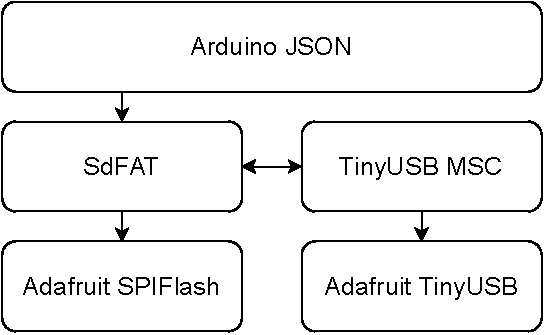
\includegraphics[height=4cm]{images/file_system_stack.pdf}
	\caption{USB and File System Library Stack}
	\label{fig:file_system_stack}
\end{figure}

\colorlet{mygray}{black!30}
\colorlet{mygreen}{green!60!blue}
\colorlet{mymauve}{red!60!blue}
\begin{lstlisting}[backgroundcolor=\color{gray!10},  
                   basicstyle=\ttfamily,
                   columns=fullflexible,
                   breakatwhitespace=false,      
                   breaklines=true,                
                   captionpos=b,                    
                   commentstyle=\color{mygreen}, 
                   extendedchars=true,              
                   frame=single,                   
                   keepspaces=true,             
                   keywordstyle=\color{blue},      
                   language=c++,                 
                   numbers=none,                
                   numbersep=5pt,                   
                   numberstyle=\tiny\color{blue}, 
                   rulecolor=\color{mygray},        
                   showspaces=false,
                   showstringspaces=false,
                   showtabs=false,                 
                   stepnumber=5,                  
                   stringstyle=\color{mymauve},    
                   tabsize=3,                      
                   title=\lstname,
                   frame=none,
                   xleftmargin = 1cm,
                   framexleftmargin = 1em]
utils_init("MONITOR");   // Initialize peripherals and file system
utils_systemConfig("system.json");   // Load system configuration
utils_startMsc();   // Start USB mass storage controller
\end{lstlisting}



\subsubsection{System Configuration}
Florian 
\subsubsection{Frame Configuration}
Florian 

\subsection{Networking}
Luca
\subsubsection{Connection}
Luca
\subsubsection{HTTP}
Luca
\subsection{FMS Frame Handler}
Luca
\subsection{Accelerometer}
Luca

\section{Utility Software Tools}
\subsection{HTTP Server}
Luca
\subsection{FMS Configuration Tool}
Flo
\subsection{FMS Data Visualizer}
Flo

\chapter{User Manual}

Description of the function of the device...

\section{Configuration}
\subsection{System}
Flo
\subsection{FMS Filter}
Flo

\section{Specifications}
Luca

\section{LED Status}
Luca

\todo[inline]{Add table: "tabular", have a look at section 4.3.3 System Configuration, how to do that}
\chapter{Summary \& Conclusion}

\section{Continuing Work}
Deployment in field, over the air firmware update, http server on onway hardware, cost reduction of hardware, accelerometer

\section{Reflection \& Project Schedule}
milestones reached as scheduled, setting up server/Usb took longer than expected, gained a lot of knowledge building a complete product.  
We developed a complete system based on our given specifications. Additional software tools were created to support our hardware in its operation. As a whole, the \acrfull{fms} monitoring system operates normally and is reliable. 
Our time management was excellent, all milestones were reached as scheduled and all functions were implemented on time. Some parts of the firmware proved to be slightly more complicated than expected which resulted in some long working days to keep up with the schedule. 

\newpage
\section{Personal Reflections}

\subsubsection{Florian Baumgartner}
Write about learning PyQt5 and Pyplot

\subsubsection{Luca Jost}
In general, this project challenged me in areas where I had no previous experience. I learned how to get an idea, with just a few requirements, to a deployable product within just a few weeks. In past projects, I had trouble with time management, so we made sure to develop a realistic timetable this time. The overall time management for this project was surprisingly easy. I was able to deliver all tasks on time. \todo{add more}

\appendix
\chapter{Dummy Appendix}

You can defer lengthy calculations that would otherwise only interrupt
the flow of your thesis to an appendix.

\backmatter

\bibliographystyle{plain}
\typeout{}
\bibliography{./sections/bibliography.bib}

\end{document}